\documentclass[11pt,a4paper]{article}
\usepackage[utf8]{inputenc}
\usepackage{amsmath}
\usepackage{amsfonts}
\usepackage{amssymb}
\usepackage[left=2cm,right=2cm,top=2cm,bottom=2cm]{geometry}


\usepackage{slashed}
\usepackage{hyperref}
\usepackage{graphicx}
\usepackage{caption}
\usepackage{float}
\usepackage{subcaption}

\renewcommand{\theequation}{\arabic{section}.\arabic{equation}}



\usepackage{ifthen}
\usepackage[dvipsnames]{xcolor}
\usepackage{tikz}


%Define color environments:

\newenvironment{DK}[1]{{\color{gray}Comment from D: #1}}

\newenvironment{DKnew}[1]{{\color{blue}NEW from D: #1}}

\newenvironment{DKres}[1]{{\color{BrickRed}RESTRUCTURED from D: #1}}




\newcommand{\dint}{  \displaystyle \int }
%%%%%%%%%%%%%%%%%%%%%%%%%%%%%%%%%%%%%%%%%%
\newcommand{\ie}{{\em i.e.} }
\newcommand{\eg}{{\em e.g.} }
\newcommand{\GeV}{{\rm GeV}}
\newcommand{\TeV}{{\rm TeV}}
\newcommand{\MeV}{{\rm MeV}}
\newcommand{\keV}{{\rm keV}}

\newcommand{\rhs}{RHS }
\newcommand{\lhs}{LHS }


\newcommand{\geff}{ g_{\rm eff} }
\newcommand{\heff}{ h_{\rm eff} }
 
 
\newcommand{\Lint}{ \mathcal{L}_{\rm int} }


\newcommand{\vev}[1]{\langle #1 \rangle}
\newcommand{\Bvev}[1]{\Bigg\langle #1 \Bigg\rangle}
\newcommand{\bvev}[1]{\Big\langle #1 \Big\rangle}




\newcommand{\lrb}[1]{\left( #1 \right)}
\newcommand{\lrsb}[1]{\left[ #1 \right]}
\newcommand{\lrBigb}[1]{\Big( #1 \Big)}
\newcommand{\lrBigsb}[1]{\Big[ #1 \Big]}
\newcommand{\lrBiggb}[1]{\Bigg( #1 \Bigg)}
\newcommand{\lrBiggsb}[1]{\Bigg[ #1 \Bigg]}

\newcommand{\lrBigcb}[1]{\Big\{ #1 \Big\}}
\newcommand{\lrBiggcb}[1]{\Bigg\{ #1 \Bigg\}}
%%%%%%%%%%%%%%%%%%%%%%%%%%%%%%%%%%%%%%%%%

%%%%%%%%%%%%%%%%%%%%%%%%%%%%%%%%%%%%%%%%%%%%%%%%%%%--Begin_refs--%%%%%%%%%%%%%%%%%%%%%%%%%%%%%%%%%%%%%%%%%%%%%%%%%%%%%%%%%%%%%%%%%%%%%%
\newcounter{NumArgs}

%Define reference to an arbitrary number of equations (\eqs{label_1,label_2....,label_n} will show eqs. ref_1, ref_2, ..., and ref_n)
\newcommand{\eqs}[1]{\setcounter{NumArgs}{0}\foreach\i in{#1}{\stepcounter{NumArgs}}%
\ifthenelse{\equal{\theNumArgs}{1}}{eq.~(\ref{#1})}%
{\ifthenelse{\equal{\theNumArgs}{2}}%
{eqs.~\foreach\i[count=\q]in{#1}{\ifthenelse{\equal{\q}{\theNumArgs}}{and (\ref{\i})}{(\ref{\i})~}}}%
{eqs.~\foreach\i[count=\q]in{#1}{\ifthenelse{\equal{\q}{\theNumArgs}}{and (\ref{\i})}{(\ref{\i}),~}}}}}


%Define reference to an arbitrary number of equations (\Eqs{label_1,label_2....,label_n} will show Eqs. ref_1, ref_2, ..., and ref_n)
\newcommand{\Eqs}[1]{\setcounter{NumArgs}{0}\foreach\i in{#1}{\stepcounter{NumArgs}}%
\ifthenelse{\equal{\theNumArgs}{1}}{Eq.~(\ref{#1})}%
{\ifthenelse{\equal{\theNumArgs}{2}}%
{Eqs.~\foreach\i[count=\q]in{#1}{\ifthenelse{\equal{\q}{\theNumArgs}}{and (\ref{\i})}{(\ref{\i})~}}}%
{Eqs.~\foreach\i[count=\q]in{#1}{\ifthenelse{\equal{\q}{\theNumArgs}}{and (\ref{\i})}{(\ref{\i}),~}}}}}


%Define reference to an arbitrary number of labels (\REF{label_1,label_2....,label_n} will show ref_1, ref_2, ..., and ref_n)
\newcommand{\refs}[1]{\setcounter{NumArgs}{0}\foreach\i in{#1}{\stepcounter{NumArgs}}%
\ifthenelse{\equal{\theNumArgs}{1}}{(\ref{#1})}%
{\ifthenelse{\equal{\theNumArgs}{2}}%
{\foreach\i[count=\q]in{#1}{\ifthenelse{\equal{\q}{\theNumArgs}}{and (\ref{\i})}{(\ref{\i})~}}}%
{\foreach\i[count=\q]in{#1}{\ifthenelse{\equal{\q}{\theNumArgs}}{and (\ref{\i})}{(\ref{\i}),~}}}}}



%Define reference to an arbitrary number of figs (\Figs{label_1,label_2....,label_n} will show ref_1, ref_2, ..., and ref_n)
\newcommand{\Figs}[1]{\setcounter{NumArgs}{0}\foreach\i in{#1}{\stepcounter{NumArgs}}%
\ifthenelse{\equal{\theNumArgs}{1}}{Fig.~(\ref{#1})}%
{\ifthenelse{\equal{\theNumArgs}{2}}%
{Figs.~\foreach\i[count=\q]in{#1}{\ifthenelse{\equal{\q}{\theNumArgs}}{and (\ref{\i})}{(\ref{\i})~}}}%
{Figs.~\foreach\i[count=\q]in{#1}{\ifthenelse{\equal{\q}{\theNumArgs}}{and (\ref{\i})}{(\ref{\i}),~}}}}}




%Define reference to an arbitrary number of "general reference" (\Gen{message}{label_1,label_2....,label_n} will show message.(ref_1), (ref_2), ..., and (ref_n)
\newcommand{\Gen}[2]{\setcounter{NumArgs}{0}\foreach\i in{#2}{\stepcounter{NumArgs}}%
	\ifthenelse{\equal{\theNumArgs}{1}}{#1.~(\ref{#2})}%
	{\ifthenelse{\equal{\theNumArgs}{2}}%
		{#1.~\foreach\i[count=\q]in{#2}{\ifthenelse{\equal{\q}{\theNumArgs}}{and (\ref{\i})}{(\ref{\i})~}}}%
		{#1.~\foreach\i[count=\q]in{#2}{\ifthenelse{\equal{\q}{\theNumArgs}}{and (\ref{\i})}{(\ref{\i}),~}}}}}


%%%%%%%%%%%%%%%%%%%%%%%%%%%%%%%%%%%%%%%%%%%%%%%%%%%--End_refs--%%%%%%%%%%%%%%%%%%%%%%%%%%%%%%%%%%%%%%%%%%%%%%%%%%%%%%%%%%%%%%%%%%%%%%



%%%%%%%-----------------------Rules-----------------------%%%%%%%
% 1. Put any new macros in macros.tex.

% 2. Section should start with:
	%\section{This is a section}\label{sec:Intro}
	%\setcounter{equation}{0}

% 3. labels for Figs should start with fig:, for equations should start with eq:, for sections with sec:, etc.
%%%%%%%--------------------------------------------------%%%%%%%




\author{Karamitros Dimitrios}
\title{This is a template for \LaTeX}
\begin{document}

\maketitle

\begin{abstract}
    Abstract goes here.
\end{abstract}


\section{This is a section}\label{sec:Intro}
\setcounter{equation}{0}

Example of an  equation is shown in \eqs{eq:example}.
%
\begin{equation}
	\int x \, dx =\dfrac{x^2}{2} \;.
\label{eq:example}
\end{equation}


This is an example of a ``generic" citation~\cite{NaBBODES}. This is a citation of an article~\cite{Darme:2019wpd}.

\subsection{Figures}\label{subsec:figs}
%
In \Figs{fig:example} you see a figure!
%
\begin{figure}[h!]
	\centering	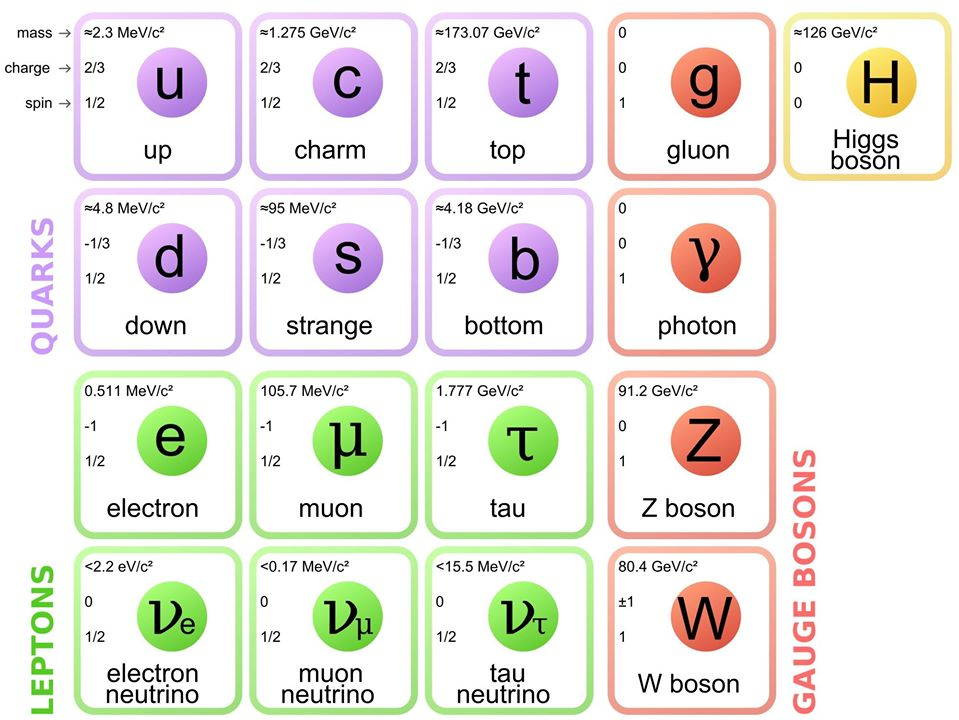
\includegraphics[width=0.8\textwidth]{figs/SM.jpg}
	\caption{This is an example of a figure}
	\label{fig:example}
\end{figure}
%


In \Figs{fig:Feyn} you see subfigures!
%
\begin{figure}[ht]
	\centering \hspace*{-1.cm}
	\begin{subfigure}[b]{0.55\textwidth}
		\centering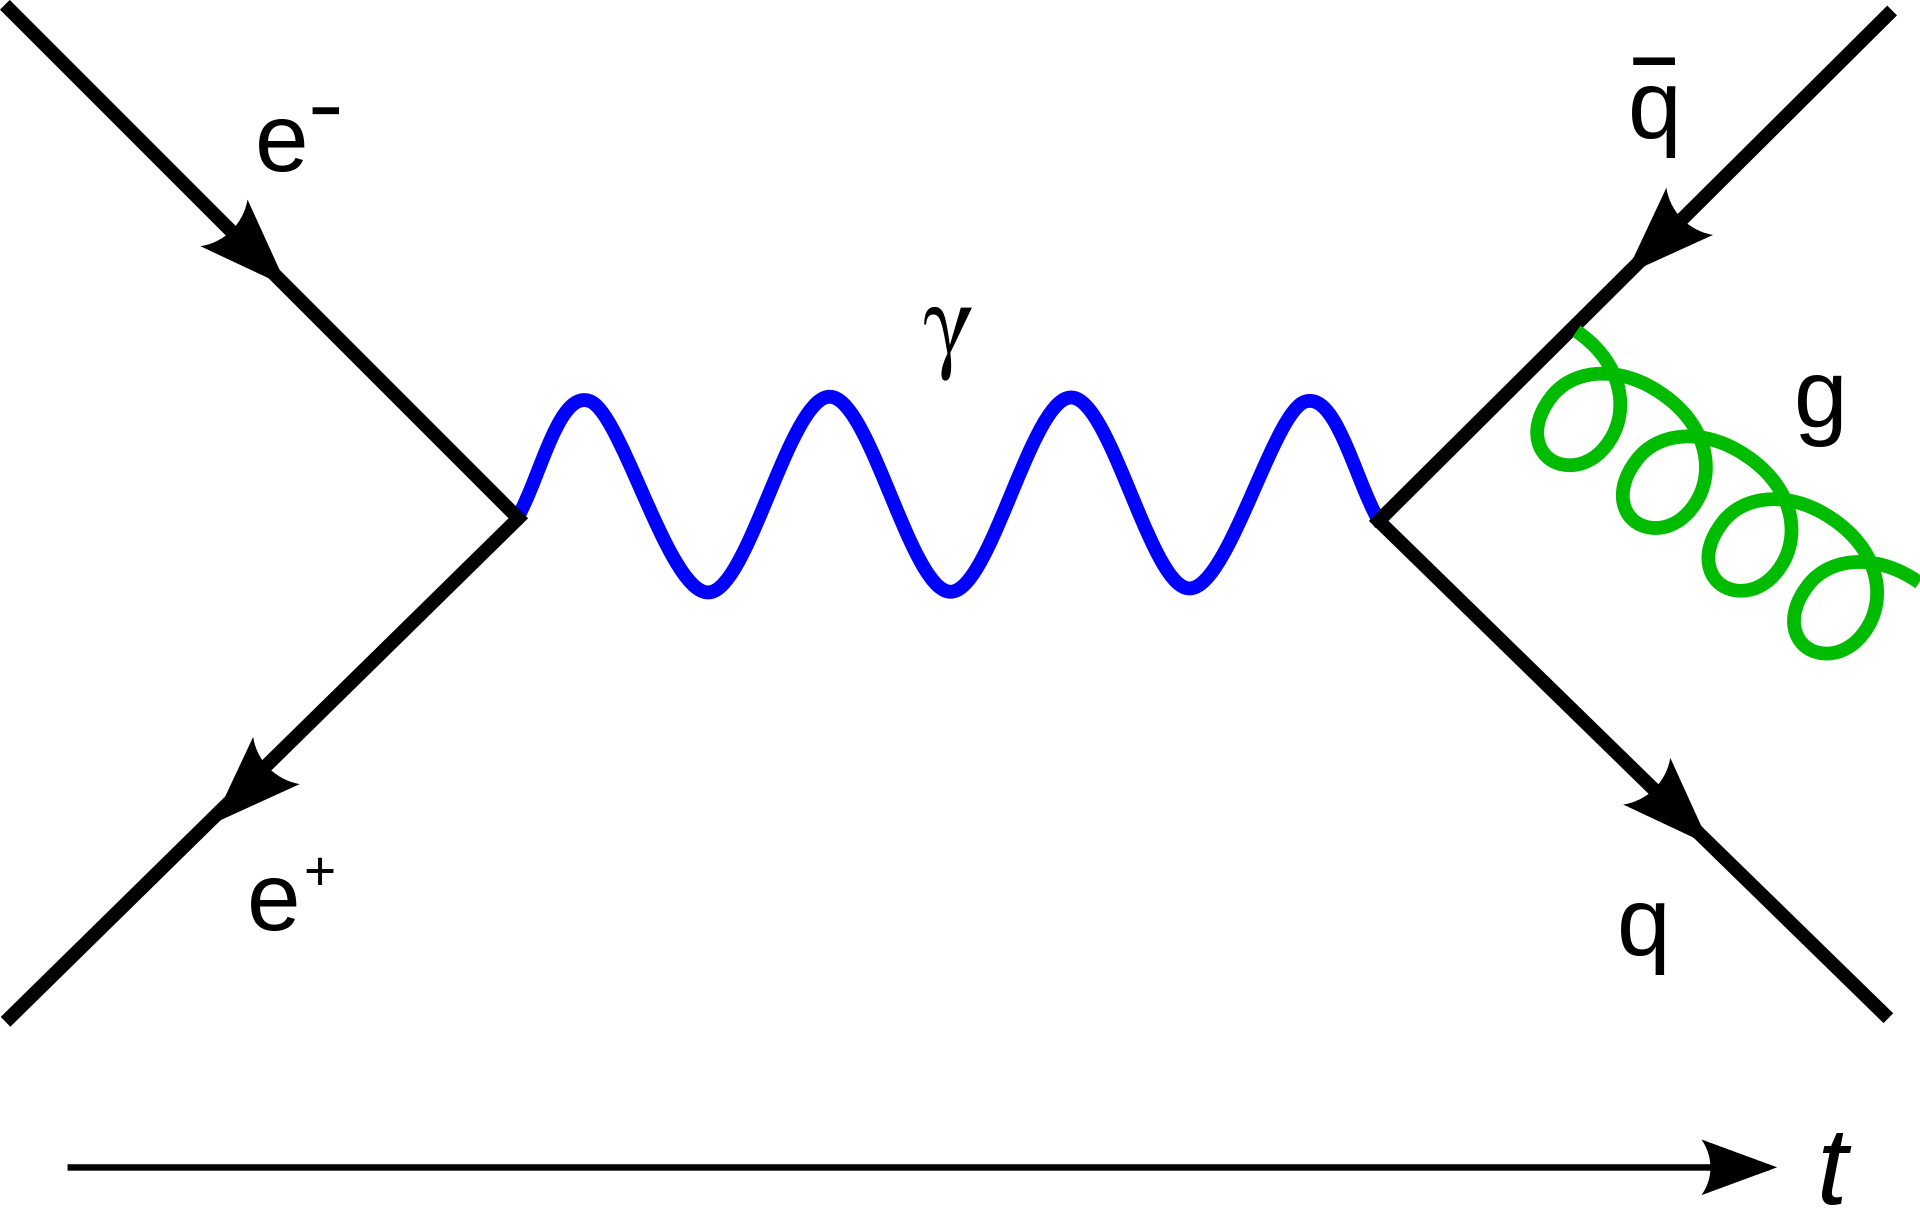
\includegraphics[width=1\textwidth ]{figs/Feyn1.png}
		\caption{\label{fig:Feyn2}}
	\end{subfigure}%
	\begin{subfigure}[b]{0.55\textwidth}
		\centering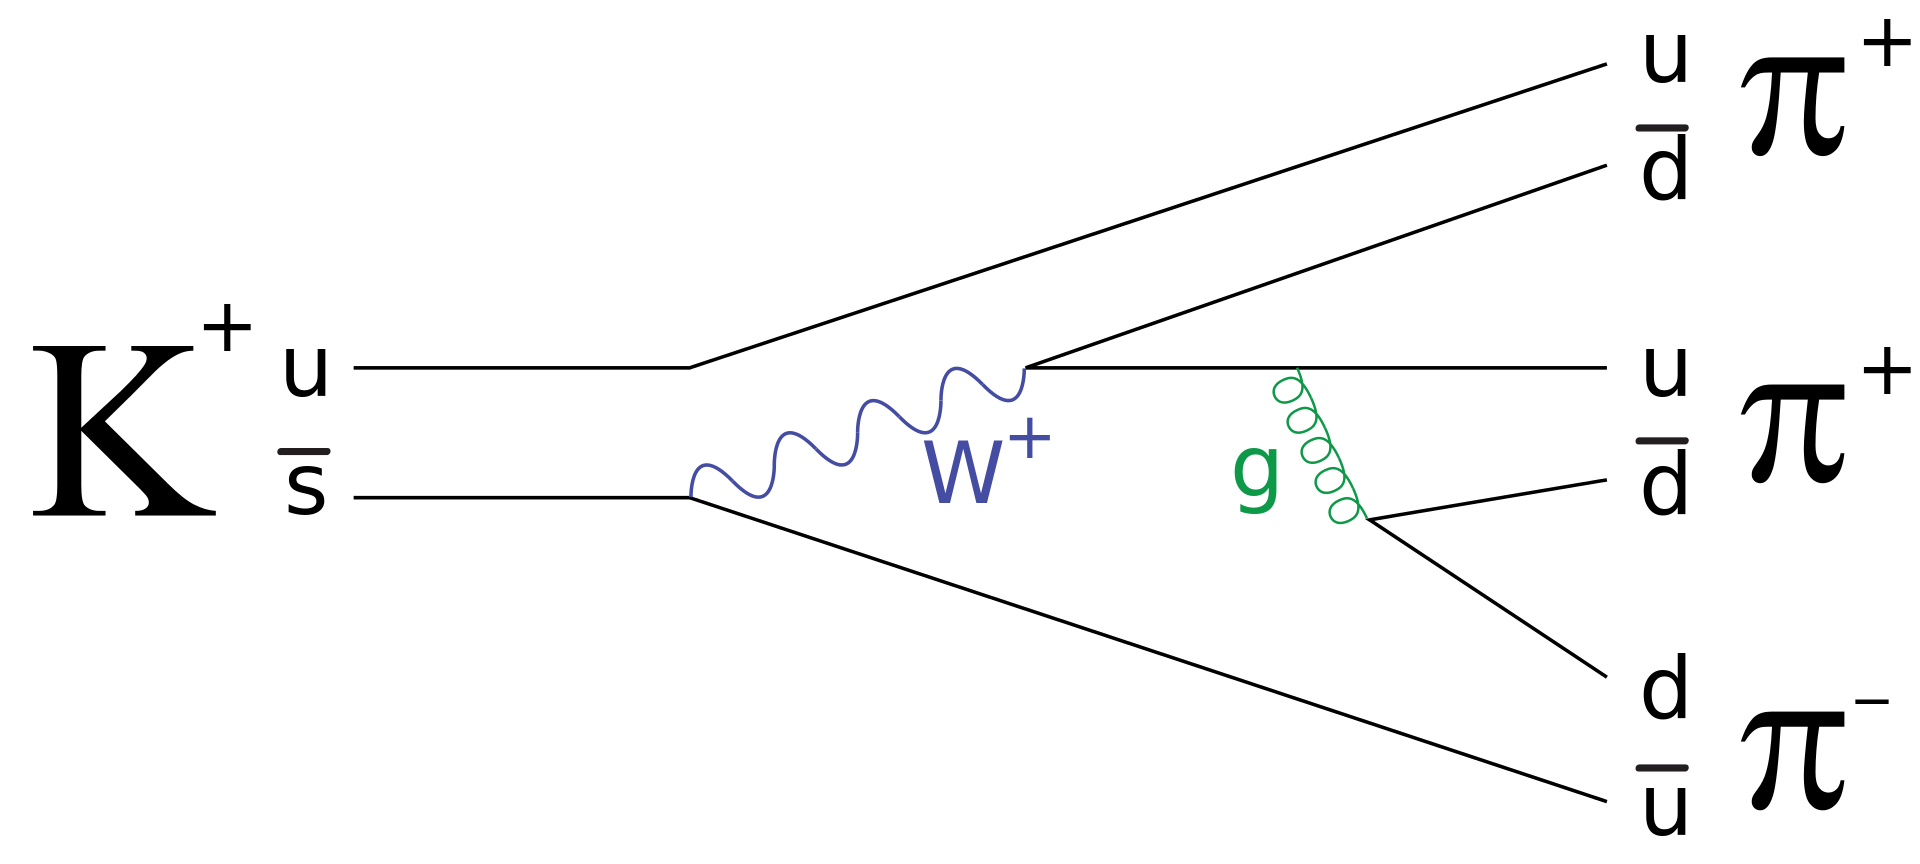
\includegraphics[width=1\textwidth]{figs/Feyn2.png}
		\caption{\label{fig:Feyn1}}
	\end{subfigure}
	\caption{Example of subfigures.}
	\label{fig:Feyn}
\end{figure}




\section{This is a section}\label{sec:Sec}
\setcounter{equation}{0}
%
The are a few macros. See the source to understand how to reference multiple equation easily as \eqs{eq:example,eq:app_eq}, as well as Figures
as \Figs{fig:example,fig:Feyn}.


%%%%%%%%%%%%%%%%%%%%%%%%%%%%%%%%%%%%%%%%
% APPENDICES
\newpage
%%%%%%%%%%%%%%%%%%%%%%%%%%%%%%%%%%%%%%%%
\setcounter{section}{0}
\section*{Appendix}
\appendix

\renewcommand{\theequation}{\Alph{section}.\arabic{equation}}
\setcounter{equation}{0}  % reset counter

%%%%%%%%%%%%%%%%%%%%%%%
\section{This is an appendix}\label{app:example}
\setcounter{equation}{0}
%
This is an appendix. Equations have different enumeration as you see in \eqs{eq:app_eq}.
%
\begin{equation}
\int x^2 \, dx =\dfrac{x^3}{3} \;.
\label{eq:app_eq}
\end{equation}




\subsection*{References you can use}

\subsubsection*{ \textbackslash eqs and \textbackslash Eqs}
References to equations:

\eqs{eq:app_eq}

\eqs{eq:app_eq,eq:example}

\eqs{eq:app_eq,eq:example,eq:example}


\Eqs{eq:app_eq}

\Eqs{eq:app_eq,eq:example}

\Eqs{eq:app_eq,eq:example,eq:example}



\subsubsection*{\textbackslash  refs}
References without ``head":

\refs{sec:Intro}

\refs{sec:Intro,sec:Intro}

\refs{sec:Intro,sec:Intro,app:example}




\subsubsection*{\textbackslash  Figs}
References to figures:

\Figs{fig:Feyn}

\Figs{fig:Feyn,fig:Feyn}

\Figs{fig:Feyn,fig:Feyn,fig:example}


\subsubsection*{\textbackslash  Gen}
References to with custom message (I know  \textbackslash refs can do the same thing):

\Gen{Figures}{fig:Feyn,fig:Feyn,fig:example}

\Gen{EquATiOnS}{eq:app_eq,eq:example,eq:example}


\newpage
%%%%%%%%%%%%%%%%%%%%%%%%%%%%%%%
\bibliography{refs}{}
\bibliographystyle{JHEP}                        

\end{document}
